%==============================================================
%\newpage
\chapter{Implementation}\label{implementationdet}

The implementation consists of two separate parts. The first contains the feature extraction and preparation of data from the audio files. The results are stored into feature files. In the second part, these feature files then have to be processed with the Big Data framework Spark to compute the similarities between songs.\\ 
Both parts are implemented in Python and can be executed on computer clusters. The source code can be found on the CD in the appendices and it can be pulled from GitHub~\cite{github-code}. Details for the usage of the Python scripts are also documented there.

\section{Underlying Hardware}

The first tests were performed on a single PC with 4 CPU cores (8 with HT) (Intel Core i7-3610QM CPU, 2.30GHz × 4) running Spark 2.4.0.\\ 
The cluster tests were performed on the ARA-cluster of the Friedrich Schiller University in Jena. 
It offers 16 compute-nodes for Spark applications with 36 CPU-cores (Dual Socket, 2 x Intel Xeon "Scalable" 6140, 2.30 GHz x 18) per node (72 with HT), and 192GB of RAM. The cluster's Spark partition is running with an older version of Spark (1.6.0). The ARA-cluster also offers a larger "Skylake" partition with 152 compute-nodes of which 36 were used to extract the audio features with. The hardware of these nodes is the same as in the Spark partition of the cluster.\\

\section{Audio Feature Extraction}\label{simmet}

So far, the required audio features as well as toolkits to extract those features from the audio data have been described and selected in Chapter~\ref{audiofeat}.
In Section~\ref{data}, different sources for audio files have been presented. Section~\ref{musly},~\ref{melsimc}, and~\ref{rhythmsimc} presented algorithms to pre-process the low-level features and use these to compute similarities. 
This section focuses on the selection of fitting datasets %to extract features from
and the performance of the feature extraction and pre-processing software implementation.  

\subsection{Test Datasets}\label{tdset}

A lot of data is needed to test the algorithms in a Big Data environment, so the Free Music Archive with its over 106000 songs is a good option for performance tests. It has to be kept in mind, that the genre distribution in the FMA dataset is quite one sided. Most of the songs are tagged as experimental, electronic, and rock. Also, this dataset may not be representative for actual popular music, a lot of the songs are live recordings with poor audio quality. %possibly influencing the results.
The 1517-Artists dataset offers 19 different genres with songs relatively evenly distributed. For an objective evaluation of the proposed algorithms, e.g., by genre recall, this dataset is ideal. For cover song detection, the covers80 dataset is included as well.
The last source used in this thesis is the private music collection. This collection is biased towards metal music, but due to the match with personal taste, it enables a subjective evaluation of the results from the implemented recommender system.
In conclusion that adds up to about 117000 songs for performance tests, from which in the end 114210 could be used (see Section~\ref{totamsong} for the details on the dropout), and about 11500 songs for a detailed evaluation of the algorithms in this thesis and the quality of the recommendations. As mentioned in Section~\ref{datasets}, all albums from the private music collections are catalogued as well, and the associated document is in the appendices. 

\begin{table}[h]
	\begin{center}
		\begin{tabular}{|c||c|}
			\hline
			FMA & 106.733 Songs\\
			\hline
			private & 8484 Songs\\
			\hline
			1517-Artists & 3180 Songs\\
			\hline
			covers80 & 164 Songs (80 originals + 84 covers)\\
			\hline
		\end{tabular}
	\end{center}
	\caption{Selected music datasets}
	\label{used_dsets}
\end{table}
\FloatBarrier

\subsection{Feature Extraction Performance}

After evaluating the different features in the last three chapters, this section only discusses the performance of the feature extraction process without going too much into the details of the code for feature pre- and post-processing, like the note estimation from the chroma features and the calculation of statistic features from the MFCCs. These additional steps were already explained in-depth in the previous chapters and are therefore left out here. The full code is in the appendices. 

\subsubsection{Librosa}

For most of the plots in Chapter~\ref{audiofeat}, the Python toolkit librosa was used because of its ease of use and very good documentation. The following code example shows the necessary steps to extract the most important features like MFCC, chromagram, beats, and onsets.
\lstset{language=Python} 
\begin{pythonCode}[frame=single,label={lst:Librosa},caption={Librosa},captionpos=b]
path = ('music/guitar2.mp3')
x, fs = librosa.load(path)
mfcc = librosa.feature.mfcc(y=x, sr=fs, n_mfcc=12)
onset_env = librosa.onset.onset_strength(x, fs, aggregate=np.median)
tempo, beats = librosa.beat.beat_track(onset_envelope=onset_env,sr=fs)
times = librosa.frames_to_time(np.arange(len(onset_env)), sr=fs, hop_length= 512)
chroma = librosa.feature.chroma_stft(x, fs)
\end{pythonCode}	

\noindent First of all an audio file is read into the variable \lstinline{x} and the sample rate \lstinline{fs} is returned by \lstinline{librosa.load(path)}. This audio file is then passed to \lstinline{librosa.feature.mfcc()} for the extraction of the MFCCs, \lstinline{librosa.onset.onset_strength()} for the onsets, and \lstinline{librosa.feature.chroma_stft()} to extract the chromagram. The onsets are also used to detect the beats and their time signatures in the song.\\
When extracting features from batches of audio files, the librosa library turned out to be very slow. For a tiny dataset of 100 songs, the extraction of just the mean, variance, and covariance of the MFCCs and the estimated notes from the chromagram took about 53 minutes on a single computer (1 CPU core used). 
For larger datasets like the 1517-Artists dataset, the feature extraction process would have taken about 28 hours and over 940 hours for the FMA dataset. 

\subsubsection{Essentia}

Moffat (et al.)~\cite{audiofeattoolb} compare different Audio feature extraction toolboxes and show that Essentia is a much faster alternative to librosa due to the underlying C++ code and provides even more features, but it is a bit less well documented and requires more effort for the implementation at the same time. In the end, the code to extract the necessary features had to be rewritten for the usage of Essentia due to the slow performance of librosa. Essentia offers two different ways to handle audio files. The first one is to use the Essentia standard library. It provides similar methods as librosa and uses an imperative programming style. The audio file has to be read, sliced and pre-processed manually. The second way is to use Essentia streaming. Basically, a network of connected algorithms is created, and they handle and schedule the "how and when" of the execution whenever a process is called. The melodic and timbral features and the beat histograms are computed with Essentia. Only the rhythm patterns and rhythm histograms are computed in a separate step, as stated below. 

\subsubsection{Essentia Standard}

In the final code for the audio feature extraction, the computation of the MFCCs and beat histogram is done with the Essentia standard library, because it offers a fast and easy way to implement the basic feature extraction tasks (see Code Snippet~\ref{lst:esss}). 
\begin{pythonCode}[frame=single,label={lst:esss},caption={Essentia standard},captionpos=b]
audio = es.MonoLoader(filename=path, sampleRate=fs)()
hamming_window = es.Windowing(type='hamming')
spectrum = es.Spectrum()
mfcc = es.MFCC(numberCoefficients=13)
mfccs = numpy.array([mfcc(spectrum(hamming_window(frame)))[1] for frame in es.FrameGenerator(audio, frameSize=2048, hopSize=1024)])
rhythm_extractor = es.RhythmExtractor2013(method="multifeature")
bpm, beats, beats_confidence, _, beats_intervals = rhythm_extractor(audio)
peak1_bpm, peak1_weight, peak1_spread, peak2_bpm, peak2_weight, peak2_spread, histogram = es.BpmHistogramDescriptors()(beats_intervals)
\end{pythonCode}
Again at first an audio file is read into the variable \lstinline{audio} by calling \lstinline{es.MonoLoader(filename=path, sampleRate=fs)()}. This audio file is then split into frames by the \lstinline{es.FrameGenerator()} for the following extraction of the MFCCs with \lstinline{mfcc(spectrum(hamming_window(frame)))[1]} for each frame. For the beat extraction the audio data gets passed to \lstinline{rhythm_extractor()}.\\

\subsubsection{Essentia Streaming}

\noindent The Essentia streaming library is used to calculate the chroma features. It eases up filtering with high- and low-pass filters. The audio signal is passed through various processing stages and ultimately results in the chroma features of the band-pass filtered audio signal. In Code Snippet~\ref{lst:essst1} the different stages get set up, e.g., the filter parameters are set by calling \lstinline{ess.HighPass(cutoffFrequency=128)} and \lstinline{ess.LowPass(cutoffFrequency=4096)}. The audio file is read by calling \lstinline{ess.MonoLoader()}.

\begin{pythonCode}[frame=single,label={lst:essst1},caption={Essentia streaming},captionpos=b]
loader = ess.MonoLoader(filename=path, sampleRate=44100)
HP = ess.HighPass(cutoffFrequency=128)
LP = ess.LowPass(cutoffFrequency=4096)
framecutter = ess.FrameCutter(frameSize=frameSize, hopSize=hopSize, silentFrames='noise')
windowing = ess.Windowing(type='blackmanharris62')
spectrum = ess.Spectrum()
spectralpeaks = ess.SpectralPeaks(orderBy='magnitude', magnitudeThreshold=0.00001, minFrequency=20, maxFrequency=3500, maxPeaks=60)
hpcp = ess.HPCP()
hpcp_key = ess.HPCP(size=36, referenceFrequency=440, bandPreset=False, minFrequency=20, maxFrequency=3500, weightType='cosine', nonLinear=False, windowSize=1.)
key = ess.Key(profileType='edma', numHarmonics=4, pcpSize=36, slope=0.6, usePolyphony=True, useThreeChords=True)
pool = essentia.Pool()
\end{pythonCode}	

\noindent In Code Snippet~\ref{lst:essst2} the audio file gets passed through the various stages. At first it gets filtered with a high- and low-pass filter, resulting in a band-pass filter operation. Then the signal gets split into frames and the chromagram (harmonic pitch class profiles, HPCP) gets extracted and stored into \lstinline{chroma}.

\begin{pythonCode}[frame=single,label={lst:essst2},caption={Essentia streaming},captionpos=b]
loader.audio >> HP.signal
HP.signal >> LP.signal
LP.signal >> framecutter.signal    
framecutter.frame >> windowing.frame >> spectrum.frame
spectrum.spectrum >> spectralpeaks.spectrum
spectralpeaks.magnitudes >> hpcp.magnitudes
spectralpeaks.frequencies >> hpcp.frequencies
spectralpeaks.magnitudes >> hpcp_key.magnitudes
spectralpeaks.frequencies >> hpcp_key.frequencies
hpcp_key.hpcp >> key.pcp
hpcp.hpcp >> (pool, 'tonal.hpcp')
essentia.run(loader)
chroma = pool['tonal.hpcp'].T
\end{pythonCode}	

\subsubsection{Essentia Performance}

The calculation with the Essentia streaming and standard library for 100 songs took less than a third of the time librosa needed. This is a significant improvement, however the Essentia library uses only one CPU core so that performance was further improved by using the Parallel Python and mpi4py library.

\subsubsection{Parallel Python}

Parallel Python is a Python module that enables the execution of Python code in parallel. On a single PC, multiple CPU cores get parts of the full filelist and compute the features fully in parallel (see Code Snippet~\ref{lst:pp}).
%\newpage
\begin{pythonCode}[frame=single,label={lst:pp},caption={Parallel Python},captionpos=b]
job_server = pp.Server()
job_server.set_ncpus(ncpus)
jobs = [ ]
for index in xrange(startjob, parts):
	starti = start+index*step
	endi = min(start+(index+1)*step, end)
	jobs.append(job_server.submit(parallel_python_process, (index, filelist[starti:endi],1,1,1,1,1)))
	gc.collect()
times = sum([job() for job in jobs])
job_server.print_stats()
\end{pythonCode}
The computation time takes on average approximately 18.6 seconds per song and processor core (assuming ideal data balancing).
\begin{equation} \label{eq:parallelp}
\text{time} = \frac{\#\text{songs}}{\#\text{CPUs}} \cdot 18.6s
\end{equation}
\noindent Using 4 CPU cores for 100 songs, the overall processing time could be reduced to about 465 seconds. 
Parallel Python also opens up the possibility to use a cluster instead of a single-node PC.\\
For convenience, every processor gets a batch of files instead of single songs. For every batch, different output files for the various features are created. The batch size determines the overall size of these feature-files. As an example, a batch size of 400 songs was chosen for the 1517-Artists dataset, which means four CPUs had to process two batches, resulting in eight different output files with the chroma feature files being the largest with about 25MB per file.\\
One problem that appeared when using Parallel Python was that the main memory usage increased over time. Neither explicit usage of the garbage collector nor the deletion of unwanted objects also could solve that problem. After processing a few hundred songs the processes eventually ran out of memory and had to be restarted. By replacing Parallel Python with mpi4py, this problem could later be solved (see Section~\ref{mpi4py}). 

\subsubsection{Rp\_extractor}

For the extraction of the rhythm patterns and rhythm histogram features as described in Section~\ref{rhythmsimc}, the "rp\_extractor" tool provided by the TU Wien was used. Although running in parallel on all CPU cores on a single node, the extraction of the features from 100 songs took about 344 seconds.

\subsubsection{Performance on a Single PC}

%The extraction of the rhythm patterns and the rhythm histogram is performed by the rp\_extractor tool. The feature extraction and processing of all the other features (beat histogram, MFCC statistics, notes and beat-aligned chromagram) had to be implemented separately and 
The performance of the different MIR toolkits is shown in Figure~\ref{perfex}. 

\begin{figure}[htbp]
	\centering
	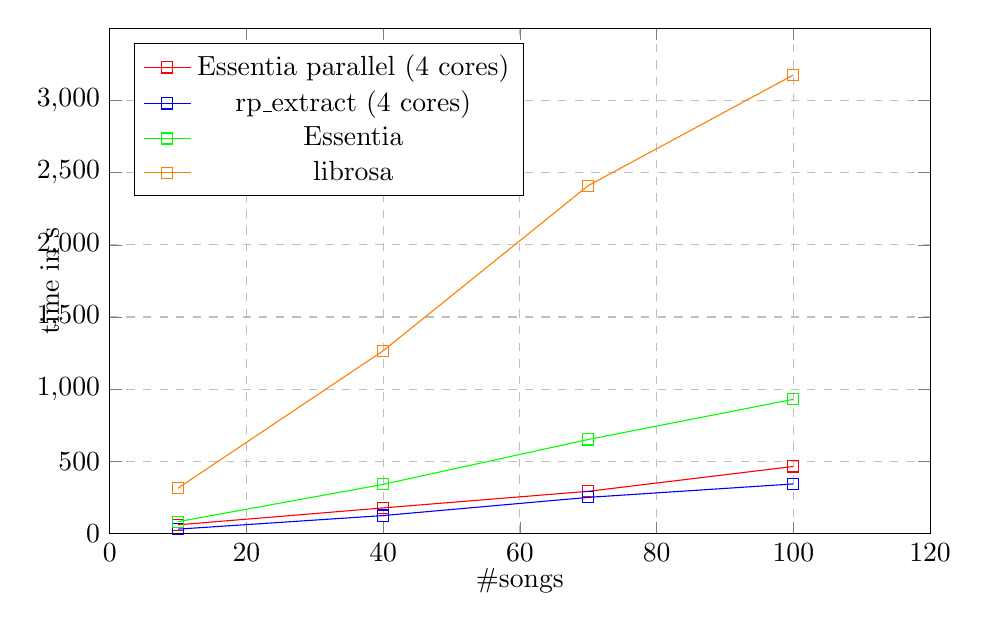
\begin{tikzpicture}
	\centering
	\begin{axis}[
	    %title={Performance of various toolkits},
		x label style={at={(axis description cs:0.5,-0.05)},anchor=north},
		y label style={at={(axis description cs:-0.05,.5)},rotate=0,anchor=south},
	    xlabel={\#songs},
	    ylabel={time in s},
	    xmin=0, xmax=120,
	    ymin=0, ymax=3500,
	    xtick={0,20,40,60,80,100,120},
	    ytick={0,500,1000,1500,2000,2500,3000},
	    legend pos=north west,
	    ymajorgrids=true,
	    grid style=dashed,
	    height=8cm,
	    width=12cm,
	    grid=major,
	]
	\addplot[
		color=red,
		mark=square,
		]
		coordinates {
		(10,61)(40,178)(70,293)(100,465)
		};
		\addlegendentry{Essentia parallel (4 cores)}
	\addplot[
	    color=blue,
	    mark=square,
	    ]
	    coordinates {
	    (10,31)(40,125)(70,251)(100,344)
	    };
	    \addlegendentry{rp\_extract  (4 cores)}
	\addplot[
	    color=green,
	    mark=square,
	    ]
	    coordinates {
		(10,83)(40,341)(70,652)(100,930)
	    };
	    \addlegendentry{Essentia}
	\addplot[
	    color=orange,
	    mark=square,
	    ]
	    coordinates {
	    (10,315)(40,1266)(70,2410)(100,3176)
	    };
	    \addlegendentry{librosa}	    
	\end{axis}
	\end{tikzpicture}
	\caption{Performance of various toolkits on a single computer}
	\label{perfex}
\end{figure}
\noindent In summary, the estimated time for the feature extraction of larger datasets on a single computer based on the performance measurements was extrapolated and is listed below, leading to the conclusion that the features for the full dataset including the FMA dataset can only be extracted with the help of a computer cluster.
\ \\
\textbf{Estimated feature extraction times}
\begin{itemize}
	\setlength\itemsep{-0.5em}
	\item 3h24min - 1517-Artists - Essentia parallel, single-node, 4 CPU cores
	\item 3h54min - 1517-Artists - rp\_extract
	\item 9h06min - private dataset - Essentia parallel, single-node, 4 CPU cores
	\item 10h24min - private dataset - rp\_extract
	\item (125h - all datasets - Essentia parallel, single-node, 4 CPU cores)
	\item (143h - all datasets - rp\_extract)
\end{itemize}

\subsubsection{Performance on a Cluster with mpi4py}\label{mpi4py}

For the extraction of the features from the audio files of the FMA dataset on the computer cluster of the Friedrich Schiller University in Jena (the "ARA-cluster"), Parallel Python had to be replaced with mpi4py (see Code Snippet~\ref{lst:mpi4py}). 
Mpi4py provides Python bindings for the Message Passing Interface standard (MPI)~\cite{mpi4py}. 
Every compute-process gets a rank number and recognizes the overall count of processes. With these two values, the file list of all audio files is split, and each process only processes its respective data. The audio files were stored in a parallel cluster file system called "beegfs"~\cite{beegfs}. Similar to the implementation using Parallel Python, every process stores the results in separate output files, each of them containing batches of 25 songs.\\

\begin{pythonCode}[frame=single,label={lst:mpi4py},caption={Mpi4py},captionpos=b]
comm = MPI.COMM_WORLD   # get MPI communicator object
size = comm.size        # total number of processes
rank = comm.rank        # rank of this process
status = MPI.Status()   # get MPI status object
files_per_part = 25
start = 0
last = len(filelist)
parts = (len(filelist) / files_per_part) + 1
step = (last - start) / parts + 1
for index in xrange(start + rank, last, size):
    if index < parts:        
        starti = start+index*step
        endi = min(start+(index+1)*step, last)
        parallel_python_process(index, filelist[starti:endi])
\end{pythonCode}

\noindent All audio files larger than 25MB were filtered out of the FMA dataset in advance, to avoid memory overflows, still leaving 102813 songs out of the 106733 songs to process. A total of 36 compute nodes were used. Every node had 192GB of RAM and 36 CPU cores (72 using hyper-threading (HT)). To increase the available memory per CPU core, only 18 CPU cores per node were used. So, overall, 648 processes were spawned. During the computation of the audio features with Essentia, 1 out of the 648 processes ran out of memory, so only 102793 out of the 102813 songs were processed in the end. For performance tests, this does not make a big difference, but for future work the feature extraction script should be adapted accordingly.\\
The ARA-cluster is managed with the help of the Slurm Workload Manager~\cite{slurm}. To submit the Essentia feature extraction script to the cluster, the following Slurm *.sbatch file was used to configure the cluster: 
\begin{lstlisting}[language=bash,frame=single,caption={Slurm *.sbatch file for feature extraction with Essentia on the ARA-cluster},captionpos=b,label={lst:sbatch}]
#!/bin/bash
#SBATCH --partition=s_standard
#SBATCH --time=08:00:00
#SBATCH -n 648
#SBATCH -N 36
#SBATCH --ntasks-per-node=18
#SBATCH --mem-per-cpu=10000
srun -n $SLURM_NTASKS --mpi=openmpi python mpi4py_ara_features.py
\end{lstlisting}
\noindent Figure \ref{featextclust} shows the performance of the feature extraction on the ARA-cluster. The extraction of the features took between 1439 seconds (fastest process) and 1950 seconds (slowest). With better balancing and messaging between the processes, the tasks could be distributed in a way where idle tasks take parts of the file list from other tasks that are still processing.\\
\noindent For the extraction of the rhythm features with the rp\_extract tool, the script of the TU Wien was adapted for usage with mpi4py as well. The same amount of processes gets spawned on the cluster (648), but each of the processes is able to make use of two CPU cores plus HT. The fastest process finished after 1657 seconds and the slowest one took 1803 seconds.

\begin{figure}[htbp]
	\centering
	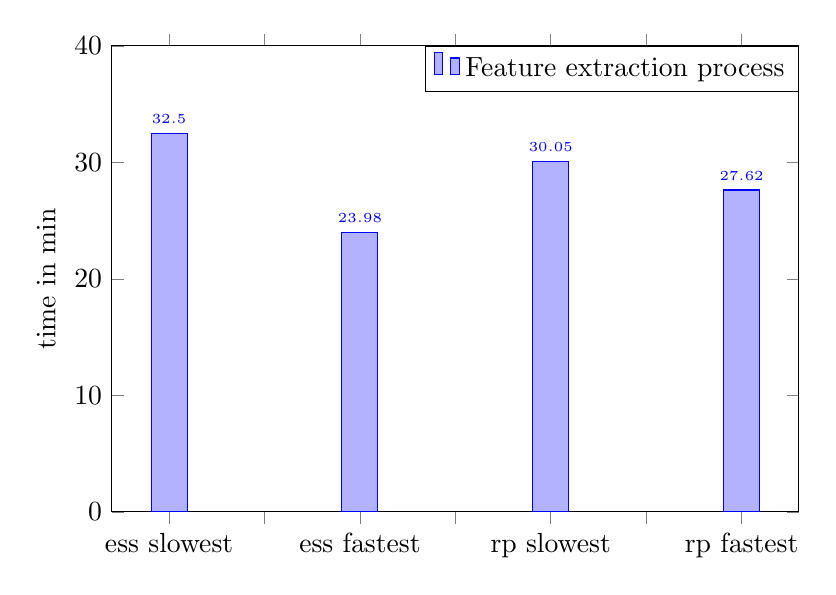
\begin{tikzpicture}
		\begin{axis}[
			width=0.85\textwidth,height=75mm,% <- added
			x tick label style={/pgf/number format/1000 sep=},
      		xticklabels={ ,  ,ess slowest, ,ess fastest, ,rp slowest, ,rp fastest}, 
			ylabel=time in min,
			ymin=0, ymax=40,
			%enlargelimits=0.05,% <- commented, default is .1
			legend style={
			at={(1,1)},
			anchor=north east,% <- changed
			%legend columns=-1% <- commented
			},
			nodes near coords,
			every node near coord/.append style={font=\tiny},
			%nodes near coords align={vertical},% <- commented, default
			ybar=0pt,%<- changed
			bar width=13pt% <- added
			]
		  \addplot
		    coordinates {(1,32.5) (2,23.98) (3,30.05) (4,27.62)};
		  \legend{Feature extraction process}
		\end{axis}
	\end{tikzpicture}
	\caption{Feature extraction of the FMA dataset on the ARA-cluster (performance)}
	\label{featextclust}
\end{figure}


\subsubsection{Total Amount of Songs}\label{totamsong}

Due to the above-mentioned filtering of audio files larger than 25MB, the out-of-memory error of one process executing the Essentia task, and since the rhythm pattern extraction script does not handle some audio file formats like Ogg Vorbis, not all features from all songs could be extracted. So, in the end, the overall count of songs from the datasets listed in Table \ref{used_dsets} where all features could be obtained is 114210.\\
